% !TeX document-id = {a39e8ab2-a52f-4b84-8569-c61394829c2b}
% !TeX TXS-program:compile = txs:///lualatex/[--shell-escape]
% !TeX TXS-program:lualatex = lualatex -synctex=1 -interaction=nonstopmode --shell-escape %.tex
\documentclass[english, a4paper]{article}

\usepackage[english]{babel}
\usepackage{inputenc}
\usepackage{xcolor}
%\usepackage[usenames, dvipsnames]{color}
\definecolor{mygray}{RGB}{198,198,198}

\usepackage{listings}
\usepackage{minted}
\setminted{breaklines, linenos, bgcolor=mygray, tabsize = 3}

\usepackage{amsthm}
\usepackage{amsmath}
%For danish setup
\usepackage{babel}

\usepackage[T1]{fontenc}
\usepackage{siunitx}				% Enheder i math mode
\usepackage[hidelinks]{hyperref} % clickable refs
\usepackage[backend=biber,style=alphabetic,hyperref]{biblatex} % Needed for bibliography
\usepackage{graphicx}
\usepackage{tabularx}
\usepackage{cleveref}



\bibliography{references} % Needed for bibliography
\graphicspath{{graphics/}}



\title{E3DSB Miniprojekt A} 
\author{	Simon Alexander Alsing, 201304202\\
			Lasse Østerberg Sangild, 20114274\\
			Tobias Kalhøj, 2015XXXXX}
\begin{document}

\maketitle

\newpage
\tableofcontents

% !TEX root = main.tex

\section{Introduction}
This project investigates the usage of different digital filters as equalizers. The filter types used are Finite Impulse Respones (FIR) and Infinite Impulse Response (IIR) filters.

FIR filters has a finite memory, and only allows an impulse response to affect the system for a FINITE amount of time.
IIR filters allows the impulse response to affect the system for an INFINITE amount of time.
There are a few key differences between the FIR and IIR.
A FIR filter can run on integer math, whereas IIR requires floating point for the calculations not to blow up. The phase is kept much more stable by using a FIR filter, compared to an IIR filter.
An IIR filter requires fewer coefficients, less memory and is generally faster than a FIR filter.

For this project we are asked to divide the filters into five different bands. Generelly speaking the human hearing is between \SI{20}{\hertz} and \SI{20}{\kilo\hertz} The five bands are taken from \href{https://en.wikipedia.org/wiki/Audio\_frequency}{here} and are adjusted to fit our range of five bands in the range of \SIrange{20}{20000}{\hertz} and are seen in \cref{tab:FiveBand}.

\begin{table}[h]
	\caption{The frequency bands filtered out.}
	\label{tab:FiveBand}
	\begin{tabularx}{\textwidth}{X X}
		\textbf{Frequency} (\si{\hertz})	& \textbf{Description} \\
		\toprule
		\numrange{0}{32}		& The lower human threshold. \\
		\numrange{32}{512}		& Rythm frequencies. \\
		\numrange{512}{2048}	& Horn like and tinny quality. Regular speach lies here. \\
		\numrange{2048}{8192}	& Labial and fricative sounds. \\
		\numrange{8192}{20000}	& Sounds of bells and ringing. \\
	\end{tabularx}
\end{table}

Lav i Matlab en audio equalizer. Equalizeren skal kunne justere niveauet på et indkommende lydsignal individuelt i fem forskellige frekvensbånd fordelt over (og dækkende) det hørbare spektrum med +/- 12 dB. Eksempelvis et bånd fra 0 hertz (eller måske 20 Hz) til 200 Hz. Herefter evt. 200-700 Hz og så fremdeles.

Der skal i opgaven indgå filtre af begge typer (FIR og IIR). Man har frie hænder til valg af designmetode. Vinduesmetoden er fin, hvis det skal foregå manuelt, - ellers er fir1.m og butter.m i Matlab gode bud.

Eksperimenter i opgaven med filterorden og knækfrekvenser. Dokumenter eksperimenterne. Equalizerens samlede impulsrespons og overføringskarakteristik (altså amplitude og fase i frekvens-domænet) skal kunne vises. Dvs. den samlede virkning af de fem filtre fra input til output.

\section{Expectations}
\label{sec:expectations}
We are going to do a few experiments comparing FIR and IIR, but also a few investigating the way either of them works.

\begin{table}
	\caption{Comparing equivalent IIR- and FIR filters.}
	\label{tab:IIRvsFIR}
	\begin{tabularx}{\textwidth}{X X X}
		Statement to test	& Expected Result	& Result \\
		\toprule
		The phase is more stable for a FIR filter & The phase of a signal is affected less by running it thorugh a FIR filter than through an IIR filter. & \\
		IIR is faster		& Using tic toc in Matlab during the filtering, IIR filter will yield a lower value. & \\
	\end{tabularx}
\end{table}

\begin{table}
	\caption{Investigation of altering the IIR coefficients.}
	\label{tab:IIRtest}
	\begin{tabularx}{\textwidth}{X X X}
		Statement to test	& Expected Result	& Result \\
		\toprule
		IIR calculation time scales exponentially with increasing coefficients. & By multiplying the coefficients by 2, 4 or 8, the calculation time increases exponentially. & \\
	\end{tabularx}
\end{table}
\newpage
<<<<<<< HEAD
\section{Frequency analysis}
\label{sec:analysis}
\subsection{Car engine}
\begin{figure}[htb]
	\centering
	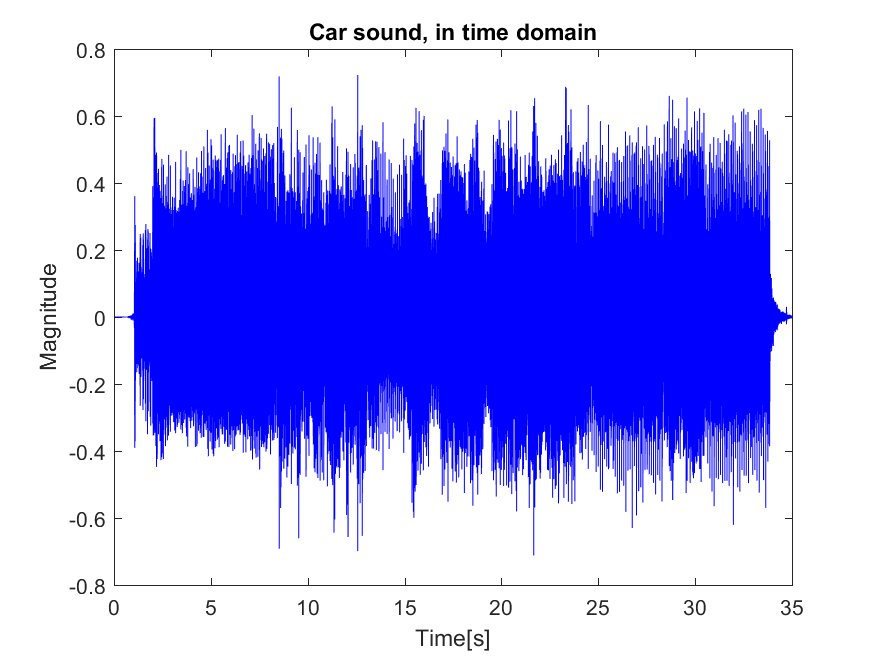
\includegraphics[width=.5\textwidth]{code/Car_figure1.png}
	\caption{The sound of a car shown in the Time Domain.}
	\label{fig:Car_figure1:1}
\end{figure}

\subsubsection{DFT}
\begin{figure}[htb]
	\centering
	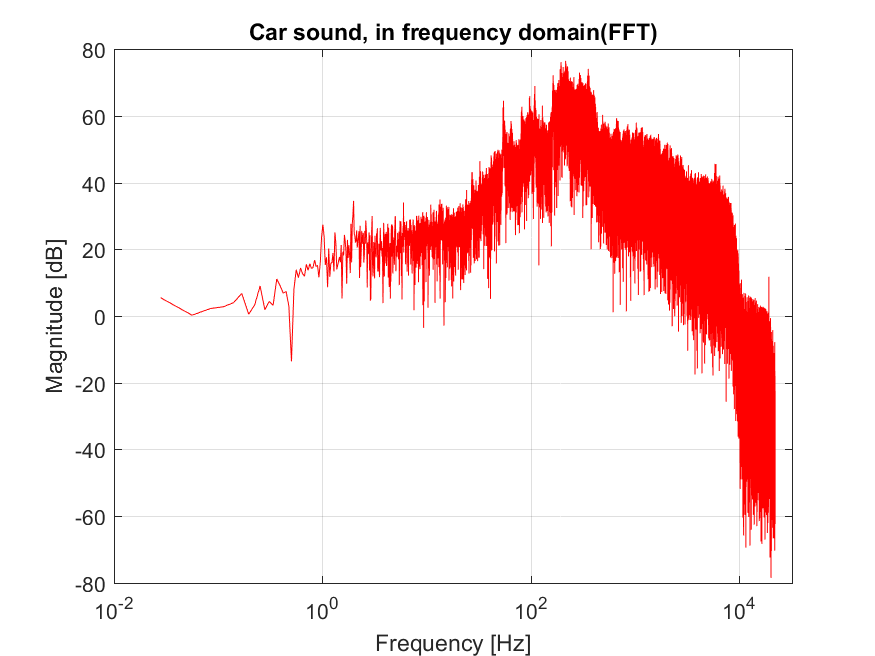
\includegraphics[width=.5\textwidth]{code/Car_figure2.png}
	\caption{The sound of a car shown in the Frequency Domain.}
	\label{fig:Car_figure2:2}
\end{figure}
=======

>>>>>>> 624490c0407af64f23ba273babf72d62fcadad27




<<<<<<< HEAD
\subsubsection{Analysis}



\subsubsection{Conclusion}

\subsection{Noise from a windmill}
\subsubsection{DFT}

\subsubsection{Analysis}

\subsubsection{Conclusion}

\subsection{EKG}
\subsubsection{DFT}

\subsubsection{Analysis}

\subsubsection{Conclusion}

\subsection{Breaking wine glass}
\subsubsection{DFT}

\subsubsection{Analysis}

\subsubsection{Conclusion}

\subsection{Music}
\subsubsection{DFT}

\subsubsection{Analysis}

\paragraph{Genre 1}

\paragraph{Genre 2}

\paragraph{Genre 3}

\paragraph{Genre 4}

\subsubsection{Conclusion}
=======

>>>>>>> 624490c0407af64f23ba273babf72d62fcadad27


\section{Energy} 
\Cref{tab:Energy} shows the energies in signals before and after the Fourier transform. It clearly shows that there is no loss of energy between the original signal and a Fourier transform, but when smoothing and windowing is applied there is a potential loss of energy.
While zero padding does not add or remove any energy from the signal.
\begin{table}[]
	\centering
	\begin{tabularx}{\textwidth}{p{2cm} | X X X X X}
		& \rotatebox{90}{\textbf{Time Domain $\times\num{e4}$}}   & \rotatebox{90}{\textbf{Frequency Domain $\times\num{e4}$}} & \rotatebox{90}{\textbf{Smooth $\times\num{e3}$}}     & \rotatebox{90}{\textbf{Zero Padding $\times\num{e4}$}}  & \rotatebox{90}{\textbf{Windowing $\times\num{e4}$}} \\
		\hline
		Windmill	& \num{4,14}	& \num{4,14}	& \num{0,521} & \num{4,14} & \num{1,79} \\

		Car Engine  & \num{3,07}	& \num{3,07}	& \num{0,686}  &	\num{3,07}  & \num{1,34}  \\

		Cheerleader & \num{13,4}	& \num{13,4}	& \num{1,29}	& \num{13,4}	& \num{7,39}  \\

		Roundtable Rival & \num{29,8}	& \num{29,8}	& \num{1,70}	& \num{29,8}	& \num{12,8}5  \\

		Micheal Jackson \newline Billie Jean & \num{16,3}	& \num{16,3}	& \num{1,73}	& \num{16,3}	& \num{6,86} \\

		Violin \newline Let It Go & \num{2,24}	& \num{2,24}	& \num{0,896}	& \num{2,24}	& \num{1,09}  \\

		Krystalglas knuses & \num{0,0115}	& \num{0,0115}	& \num{0,155}	& \num{0,0115}	& \num{0,000265} \\

		EKG & \num{2,05}	& \num{2,05}	& \num{0,626}	& \num{2,05}	& \num{0,729}
	\end{tabularx}
	
	\caption{Energy of the different signals shown in \si{\joule}.}
	\label{tab:Energy}
\end{table}

\section{Discussion}

Skalering --> Vi kan ikke bruge frekvenser højere end nyquits frekvens ?
Korrekte frekvensbins?

\section{Conclusion}

\printbibliography
\section{appendix}



\end{document}
